A seismograph in a house records the ground moving back and forth during an earthquake (see the graph below). Take the motion as harmonic.

\begin{center}
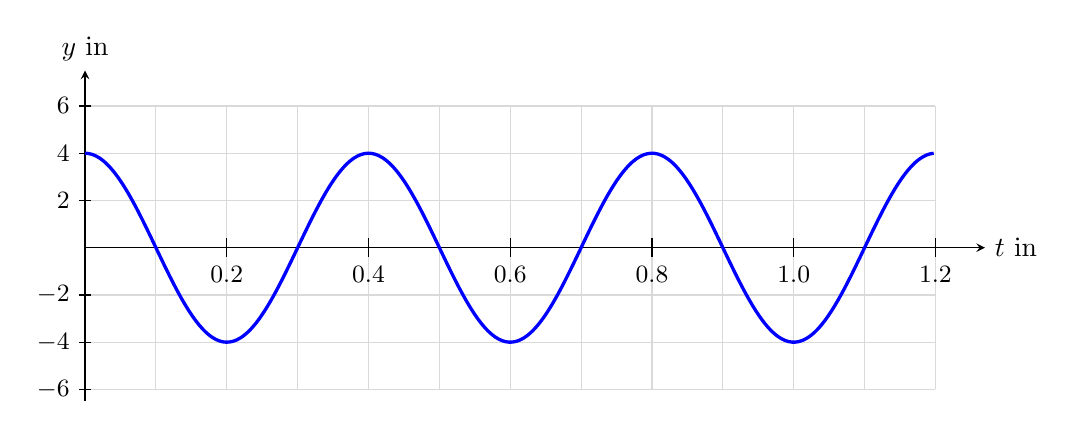
\begin{tikzpicture}[xscale=9, yscale=0.3, >=stealth]
 \draw[black!15] (0,-6) grid[xstep=0.1, ystep=2] (1.2,6);
 \draw[->] (0,0) -- (1.27,0) node[right] {$t$ in \si{\second}};
 \draw[->] (0,-6.5) -- (0,7.5) node[above] {$y$ in \si{\cm}};
 \foreach \xt in {0.2,0.4,0.6,0.8,1.0,1.2} \draw (\xt,0.4) -- (\xt,-0.4) node[below] {\small $\xt$};
 \foreach \yt in {-6,-4,-2,2,4,6} \draw (0.008,\yt) -- (-0.008,\yt) node[left] {\small $\yt$};
 \draw[very thick, blue, domain=0:1.2, samples=241, smooth] plot (\x, {4*cos(900*\x)});
\end{tikzpicture}
\end{center}

\begin{abcliste}
\abc
What is the largest acceleration of the ground?

\abc
How many times $g$ is that? (Buildings are at risk from about \rdO\,$g$.)
\end{abcliste}
